\subsection{LWM2M: CoAP and HTTP with Leshan}


LWM2M is the fundamental ingredient in the broker. It provides a REST API for both CoAP and HTTP which can both be modified to serve the needs of the system. Leshan operates with a server/client infrastructure. Thus the broker runs a server module and other devices connecting to it use a client module. The android app and the cloud service take advantage of the HTTP protocol and the end-device uses the CoAP protocol.

\begin{figure}[h]
	\begin{center}
		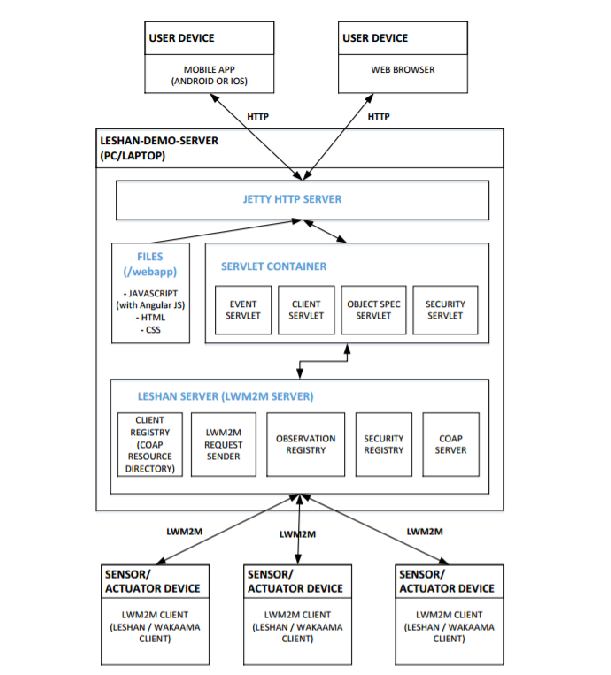
\includegraphics[width=1.3\linewidth]{img/LeshanArc}
		\caption{Architecture of Leshan Server used in implementation} 
		\label{fig:fig3}
	\end{center}
\end{figure}

\subsection{User app: Android} 
User App is used to update the light settings of the the user. The settings can be accessed only after logging in with the userId and password. The details are sent to the broker using HTTP protocol(GET). The broker receives the information of all the userID's and their corresponding passwords from cloud service during the "Set User Account" phase. While the intended application is to get the change the corresponding user light settings when logged in, due to a misunderstanding we implemented an which could modify the current light settings of any client active at that moment. Hence any user when logged in with correct details can modify the light settings(provided the client has  a light device) of all the clients active at that point of time.

\begin{figure}[h]
	\begin{center}
		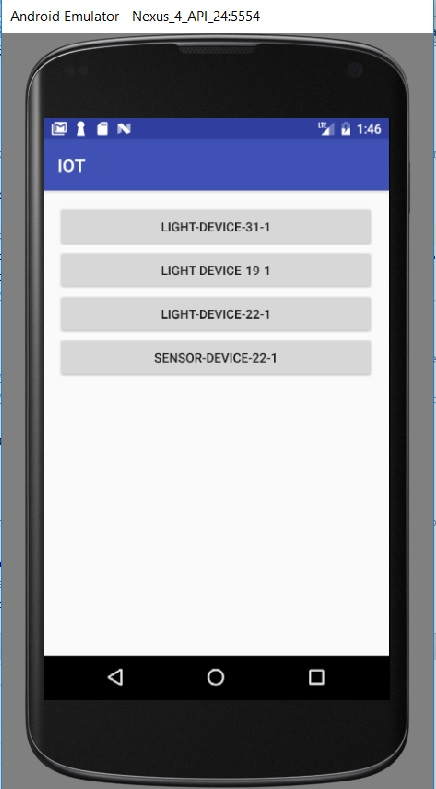
\includegraphics[width=.7\linewidth]{img/android1}
		\caption{Client Details in android App}
		\label{fig:fig3}
	\end{center}
\end{figure}


\begin{figure}[h]
	\begin{center}
		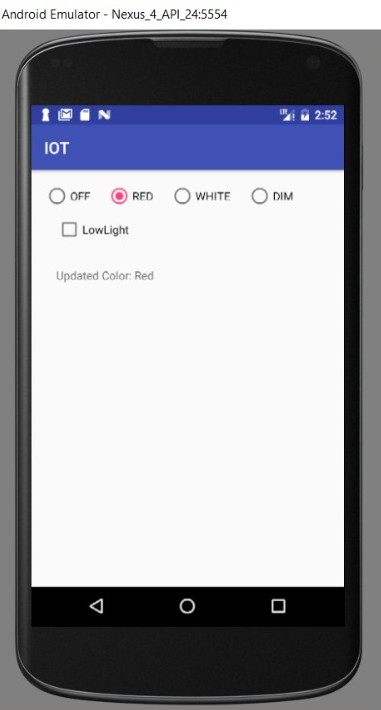
\includegraphics[width=.7\linewidth]{img/androidapp}
		\caption{Updating Light Values from User App }
		\label{fig:fig4}
	\end{center}
\end{figure}



Note:During the interactions between user app and the broker the IP address of broker is manually set during the initialization phase of the app. No service discovery is used in this case.